%%%%%%%%%%%%%%%%%%%%%%%%%%%%%%%%%%%%%%%%%%%%%%%%%%%%%%%%%%
\frame {\frametitle{We live in a world of data}
%%%%%%%%%%%%%%%%%%%%%%%%%%%%%%%%%%%%%%%%%%%%%%%%%%%%%%%%%%
  \begin{figure}[h]
    \centering
    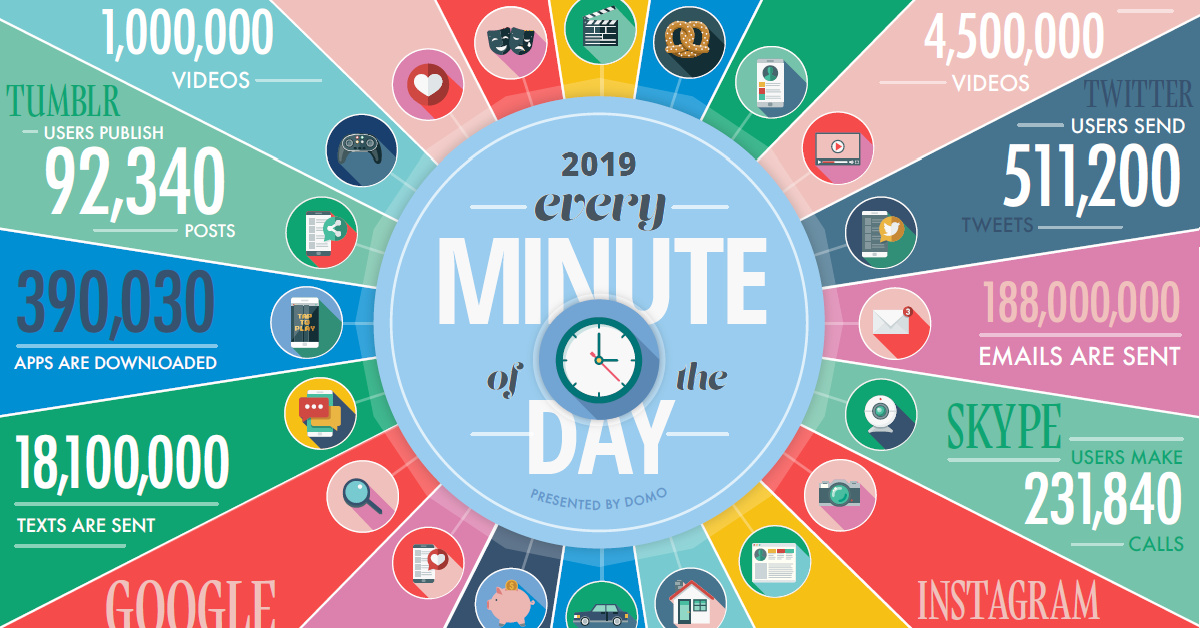
\includegraphics[scale=0.25]{./Figures/big-data-graphic}
    \caption{Data deluge.}
    \label{fig:hdfs}
  \end{figure}
}


%%%%%%%%%%%%%%%%%%%%%%%%%%%%%%%%%%%%%%%%%%%%%%%%%%%%%%%%%%
\frame {\frametitle{Big Data}
%%%%%%%%%%%%%%%%%%%%%%%%%%%%%%%%%%%%%%%%%%%%%%%%%%%%%%%%%%
\begin{itemize}

    \item \textbf{Big data is defined as large pools of data that can be captured, communicated, aggregated, stored, and analyzed.}

    \item \textbf{Data continues to grow}
	\begin{figure}[h]
		\centering
		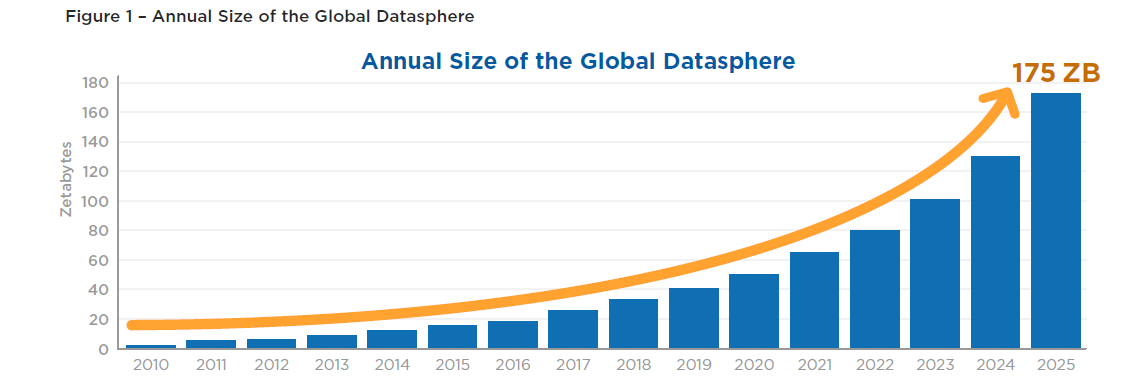
\includegraphics[scale=0.25]{./Figures/IDC_DataSphere}
		\caption{Global datasphere}
		\label{fig:hdfs}
	\end{figure}
	
    \item \textbf{Applications are becoming data intensive}
	\begin{itemize}
		\item More data leads to better accuracy
		\item With more data, accuracy of different algorithms converges
	\end{itemize}
	
\end{itemize}
}

%%%%%%%%%%%%%%%%%%%%%%%%%%%%%%%%%%%%%%%%%%%%%%%%%%%%%%%%%%
\frame {\frametitle{Let's look at your data.}
%%%%%%%%%%%%%%%%%%%%%%%%%%%%%%%%%%%%%%%%%%%%%%%%%%%%%%%%%%
  \begin{figure}[h]
    \centering
    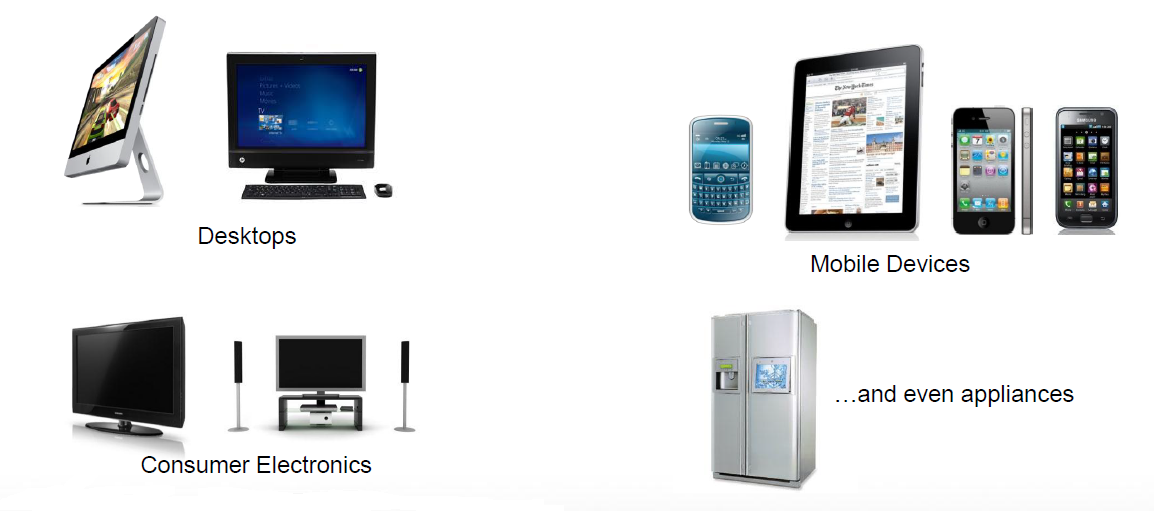
\includegraphics[scale=0.5]{./Figures/devices}
    \label{fig:hdfs}
  \end{figure}
  
 \begin{colorblock}{blue}{lightblue}{ }
  \begin{center}
    \large \textbf{\texttt{You want to access, shared, process your data \\from all your devices, anytime, anywhere.}}
  \end{center}
  \end{colorblock}
}

%%%%%%%%%%%%%%%%%%%%%%%%%%%%%%%%%%%%%%%%%%%%%%%%%%%%%%%%%%
\frame {\frametitle{How will we manage all this data?}
%%%%%%%%%%%%%%%%%%%%%%%%%%%%%%%%%%%%%%%%%%%%%%%%%%%%%%%%%%
\begin{itemize}

    \item \textbf{Manage it ourselves?}
    \begin{itemize}
      \item How do we store it? 
	  \item How do we share it? 
	  \item How can we enable access to it from any place?
	  \item How do we process all of it?
	  \item How do we secure it?
	  \item ....
    \end{itemize}
	
	\item \textbf{What if it is managed by someone else?}
    \begin{itemize}
      \item Someone provides a management ``service'' 
	  \item You pay a subscription for this ``service''
    \end{itemize}
	
\end{itemize}
}

%%%%%%%%%%%%%%%%%%%%%%%%%%%%%%%%%%%%%%%%%%%%%%%%%%%%%%%%%%
\frame {\frametitle{Utility--Product--Service lifecycle (1)}
%%%%%%%%%%%%%%%%%%%%%%%%%%%%%%%%%%%%%%%%%%%%%%%%%%%%%%%%%%
  \begin{figure}[h]
    \centering
    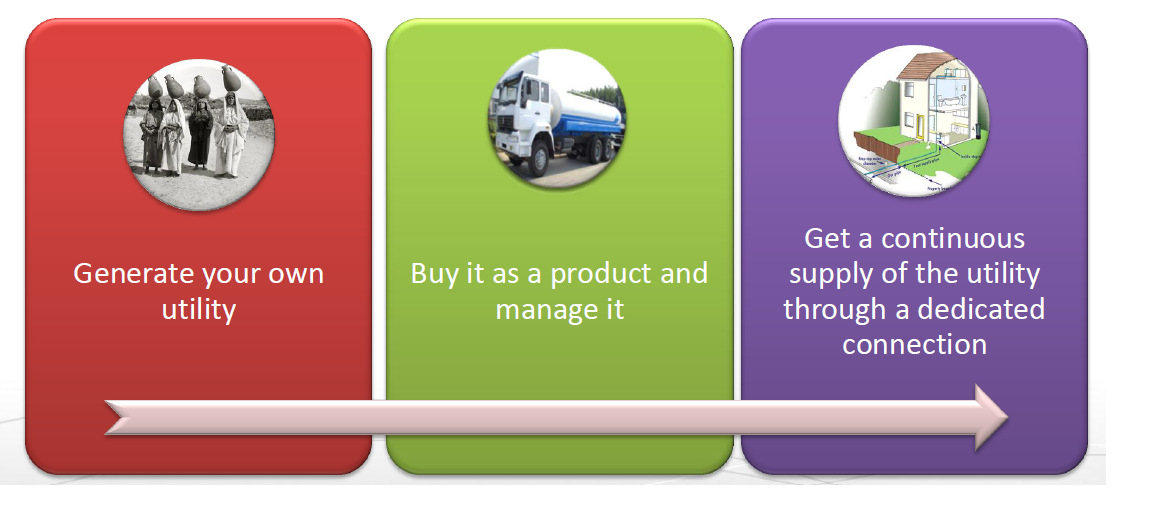
\includegraphics[scale=0.5]{./Figures/water-utility}
    \label{fig:hdfs}
  \end{figure}
}

%%%%%%%%%%%%%%%%%%%%%%%%%%%%%%%%%%%%%%%%%%%%%%%%%%%%%%%%%%
\frame {\frametitle{Utility--Product--Service lifecycle (2)}
%%%%%%%%%%%%%%%%%%%%%%%%%%%%%%%%%%%%%%%%%%%%%%%%%%%%%%%%%%
  \begin{figure}[h]
    \centering
    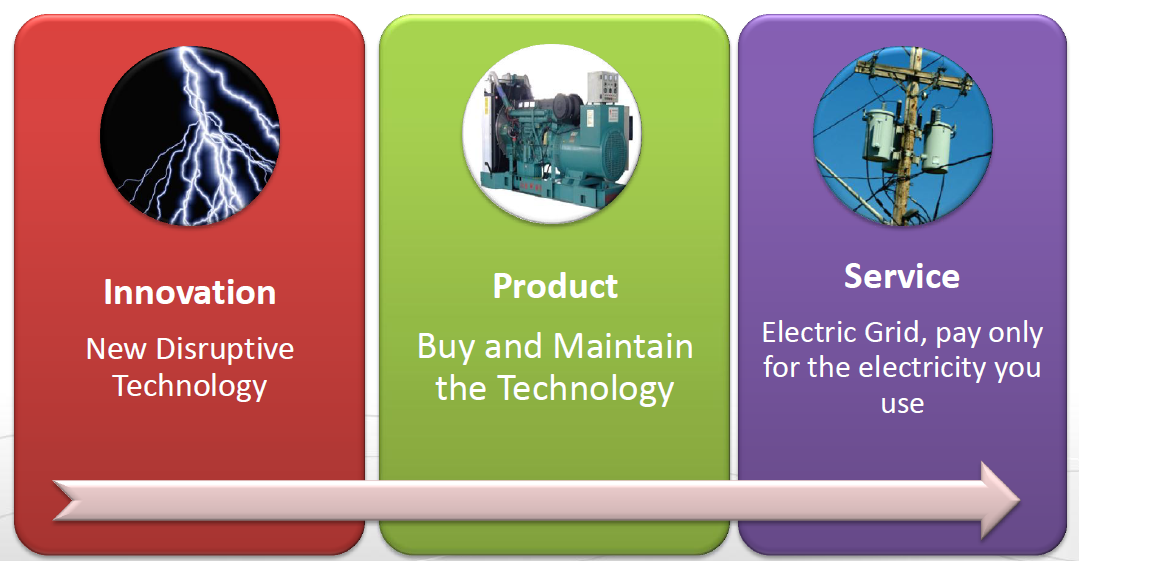
\includegraphics[scale=0.5]{./Figures/electricity-utility}
    \label{fig:hdfs}
  \end{figure}
}

%%%%%%%%%%%%%%%%%%%%%%%%%%%%%%%%%%%%%%%%%%%%%%%%%%%%%%%%%%
\frame {\frametitle{Generalizing the lifecycle}
%%%%%%%%%%%%%%%%%%%%%%%%%%%%%%%%%%%%%%%%%%%%%%%%%%%%%%%%%%
  \begin{figure}[h]
    \centering
    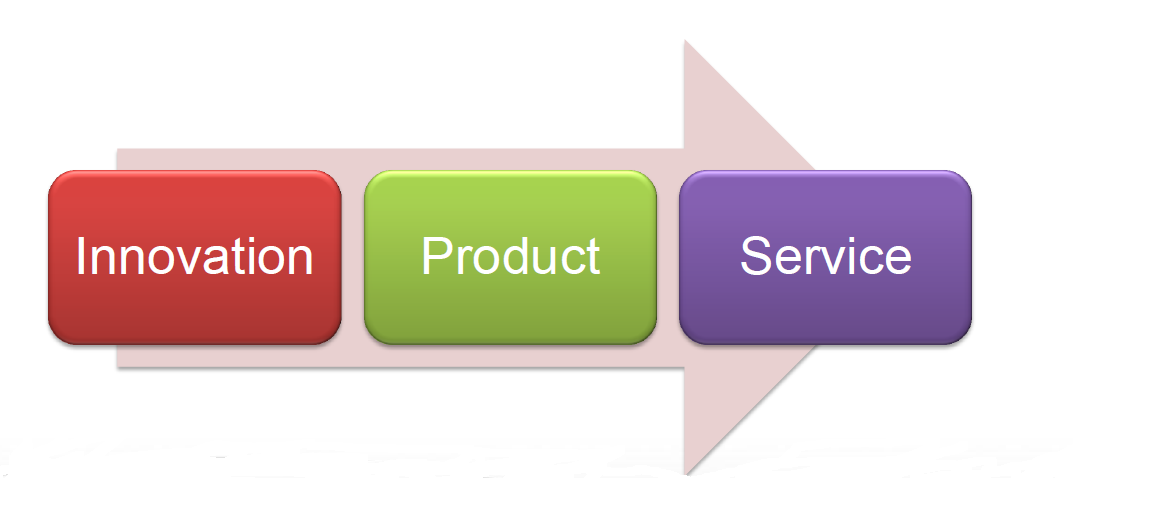
\includegraphics[scale=0.5]{./Figures/generalizing-lifecycle}
    \label{fig:hdfs}
  \end{figure}
}


%%%%%%%%%%%%%%%%%%%%%%%%%%%%%%%%%%%%%%%%%%%%%%%%%%%%%%%%%%
\frame {\frametitle{Cloud Computing}
%%%%%%%%%%%%%%%%%%%%%%%%%%%%%%%%%%%%%%%%%%%%%%%%%%%%%%%%%%

\begin{itemize}
	\item Transformation of IT from a product to a service
\end{itemize}

  \begin{figure}[h]
    \centering
    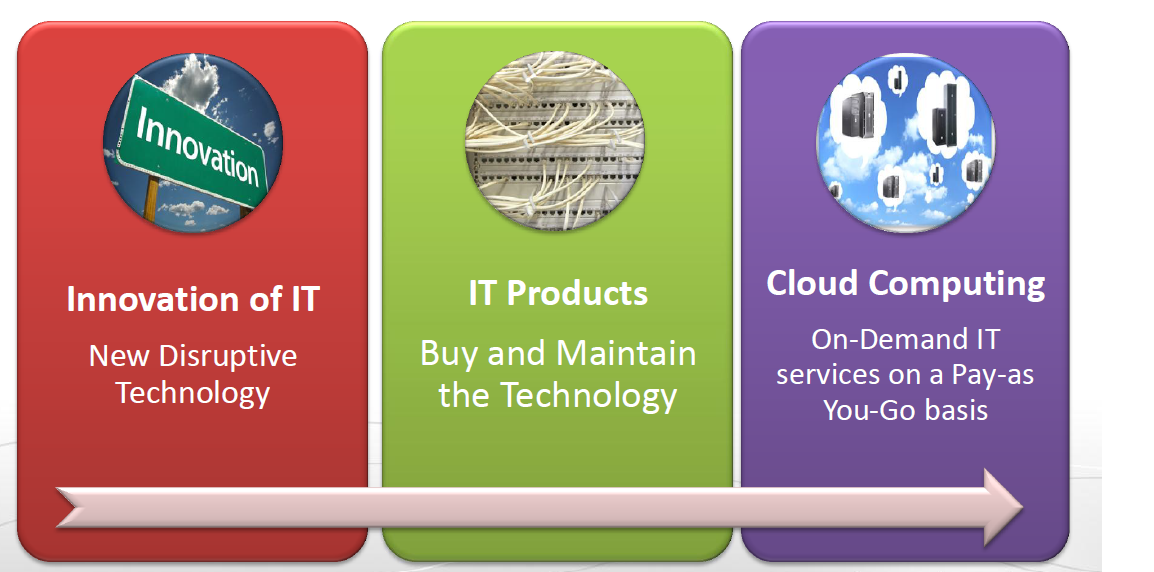
\includegraphics[scale=0.5]{./Figures/it-transformation}
    \label{fig:hdfs}
  \end{figure}
}

%%%%%%%%%%%%%%%%%%%%%%%%%%%%%%%%%%%%%%%%%%%%%%%%%%%%%%%%%%
\frame {\frametitle{How did IT transformation happen?}
%%%%%%%%%%%%%%%%%%%%%%%%%%%%%%%%%%%%%%%%%%%%%%%%%%%%%%%%%%
\begin{itemize}
	\item Requirements to transform IT
	
	\begin{itemize}
		\item Connectivity to move data
		\item Interactivity for seamless interface
		\item Reliability against failures
		\item Acceptable performance 
		\item Ease of programmability for developing new services
		\item Manageability for Big Data
		\item Pay-as-you-go to avoid capital investment		
		\item Scalability and elasticity for changing needs
	\end{itemize}
	
\end{itemize}
}

%%%%%%%%%%%%%%%%%%%%%%%%%%%%%%%%%%%%%%%%%%%%%%%%%%%%%%%%%%
\frame {\frametitle{Supporting technologies}
%%%%%%%%%%%%%%%%%%%%%%%%%%%%%%%%%%%%%%%%%%%%%%%%%%%%%%%%%%
\begin{itemize}
	\item Cloud computing is a combination of technologies
	
	\begin{itemize}
		\item Connectivity to move data => \textbf{Networked systems}
		\item Interactivity for seamless interface => \textbf{Web 2.0 and HCI} 
		\item Reliability against failures => \textbf{Dependable systems}
		\item Acceptable performance => \textbf{Parallel and distributed systems}
		\item Ease of programmability for developing new services => \textbf{Programming languages}
		\item Manageability for Big Data  => \textbf{Storage systems}
		\item Pay-as-you-go to avoid capital investment	=> \textbf{Utility computing \& economics}	
		\item Scalability and elasticity for changing needs => \textbf{Virtualization}
	\end{itemize}
	
\end{itemize}
}

%%%%%%%%%%%%%%%%%%%%%%%%%%%%%%%%%%%%%%%%%%%%%%%%%%%%%%%%%%
\frame {\frametitle{Formal definition}
%%%%%%%%%%%%%%%%%%%%%%%%%%%%%%%%%%%%%%%%%%%%%%%%%%%%%%%%%%

\begin{figure}[h]
	\centering
	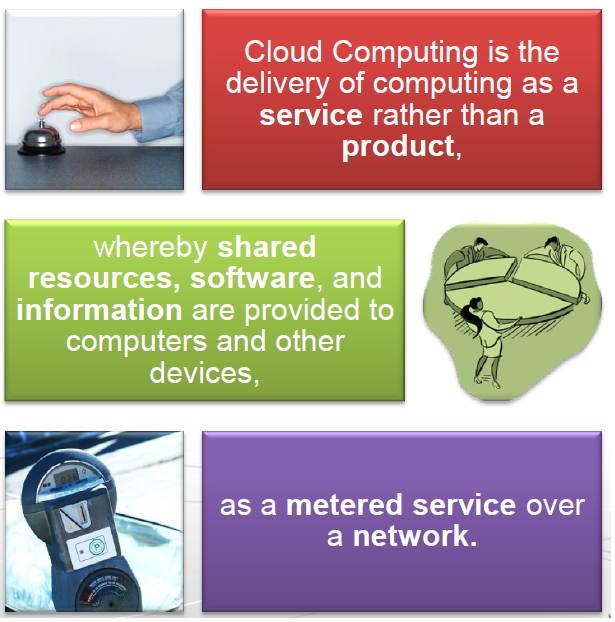
\includegraphics[scale=0.5]{./Figures/cloud-definition}
	\label{fig:hdfs}
\end{figure}
}

%%%%%%%%%%%%%%%%%%%%%%%%%%%%%%%%%%%%%%%%%%%%%%%%%%%%%%%%%%
\frame {\frametitle{Why Cloud Computing?}
%%%%%%%%%%%%%%%%%%%%%%%%%%%%%%%%%%%%%%%%%%%%%%%%%%%%%%%%%%
\begin{figure}[h]
	\centering
	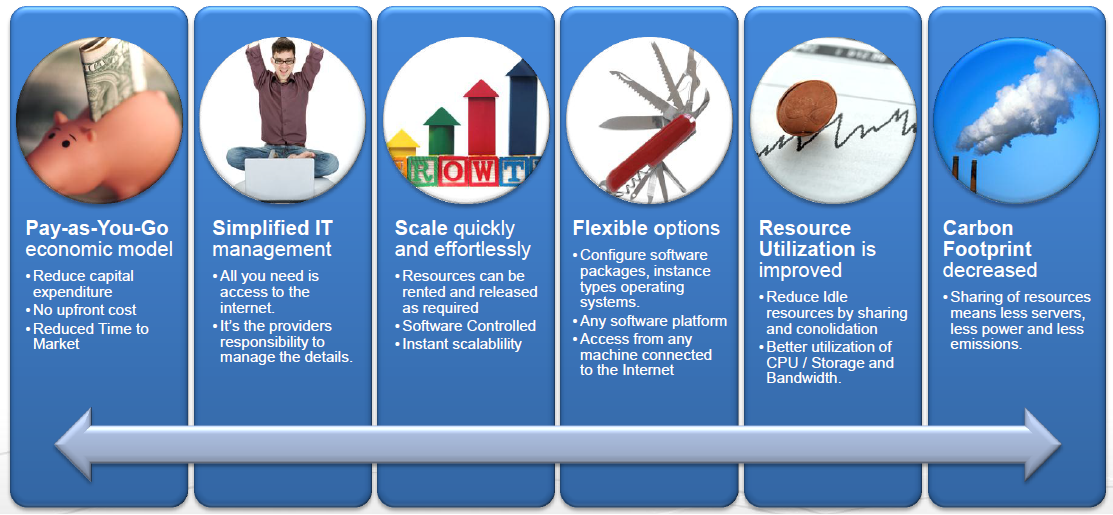
\includegraphics[scale=0.6]{./Figures/why-cloud}
	\label{fig:hdfs}
\end{figure}
}


%%%%%%%%%%%%%%%%%%%%%%%%%%%%%%%%%%%%%%%%%%%%%%%%%%%%%%%%%%
\frame {\frametitle{Applications enabled by cloud computing}
%%%%%%%%%%%%%%%%%%%%%%%%%%%%%%%%%%%%%%%%%%%%%%%%%%%%%%%%%%
\begin{itemize}
	\item High-growth applications
	\begin{itemize}
		\item When you startup gains traction, can you keep up?
		\item Friendster(2001): Could not keep up with user growth
		\item Facebook (2006): \$Billion company today			
		\item Airbnb, Uber, Expedia, ...			
	\end{itemize}

	\item Aperiodic applications
	\begin{itemize}
		\item How do you deal with sudden load peaks?
		\begin{itemize}
			\item Amazon Prime Day: Aurora cloud database processed 148 billion transactions, stored 609 terabytes of data, and transferred 306 terabytes of data
			\item Flipkart: Website crashed on their ``Big Billion Day'' sale
		\end{itemize}
		
		\item If you design for peak, how do you deal with low loads?
		\begin{itemize}
			\item Amazon normal day: 1.3 billion transactions
		\end{itemize}		
	\end{itemize}	
\end{itemize}
}

%%%%%%%%%%%%%%%%%%%%%%%%%%%%%%%%%%%%%%%%%%%%%%%%%%%%%%%%%%
\frame {\frametitle{Applications enabled by cloud computing(2)}
%%%%%%%%%%%%%%%%%%%%%%%%%%%%%%%%%%%%%%%%%%%%%%%%%%%%%%%%%%
\begin{itemize}
	\item On-off applications
	\begin{itemize}
		\item Scientific simulation using 1000s of computers
		\begin{itemize}
			\item DNA Nexus and Baylor college of medicine analyzed DNA of more than 14,000 individuals
			\item 2.4 million core-hours of computational time, 440 TB of results, 1PB of storage
		\end{itemize}		
		\item Why not rent computing time to run such one-off experiments?
	\end{itemize}
	
	\item Periodic applications
	\begin{itemize}
		\item Stock market analysis
		\begin{itemize}
			\item Mine market data during day
			\item Analyze data during night
			\item Different computational requirements at different times
		\end{itemize}
		
		\item Dynamic, flexible infrastructure can reduce costs, improve performance
	\end{itemize}
\end{itemize}
}